\documentclass{beamer}
%\documentclass[handout]{beamer}
\usepackage[latin1]{inputenc}


%%%%%%%%%%%%%
%% THEMES w/o navigaton
%\usetheme{default}
%\usetheme{Madrid}
%\usetheme{Pittsburgh}
\usetheme{Boadilla}

%%%%%%%%%%%%%
%% THEMES w/ tree navigation
%\usetheme{Antibes}

%%%%%%%%%%%%%
%% THEMES w/ TOC sidebar
%\usetheme{Berkeley}

%%%%%%%%%%%%%
%% THEMES w/ miniframe navigation
%\usetheme{Berlin}
%\usetheme{Darmstadt}
%\usetheme{Ilmenau}
%\usetheme{Singapore}
%\usetheme{Frankfurt}

%%%%%%%%%%%%%
%% THEMES w/ section/subsection titles
%\usetheme{Copenhagen}
%\usetheme{Warsaw}


%%%%%%%%%%%%%%%

\usecolortheme{beaver}

\usepackage{tikz}
\usetikzlibrary{arrows}

\DeclareMathOperator*{\argmax}{arg\,max}
\DeclareMathOperator*{\argmin}{arg\,min}
%\DeclareMathOperator*{\Em}{E_w(x=x^{(m)},h)}
\DeclareMathOperator*{\Em}{E_w(x^{(m)},h)}
\DeclareMathOperator*{\E}{E_w(x,h)}
\DeclareMathOperator*{\nw}{\nabla_{w_{ij}}}
\newcommand{\btheta}{\boldsymbol \theta }
\newcommand{\bi}{\begin{itemize}}
\newcommand{\ei}{\end{itemize}}
\newcommand{\be}{\begin{enumerate}}
\newcommand{\ee}{\end{enumerate}}


\setbeamertemplate{footline}{\hfill\insertframenumber/\inserttotalframenumber}
%\setbeamertemplate{footline}[page number]

\makeatletter
\def\blfootnote{\xdef\@thefnmark{}\@footnotetext}
\makeatother

\title[Deep Learning]{Deep Learning \& Neural Networks\\Lecture 1}
\author[K. Duh]{Kevin Duh}
\institute[]{Graduate School of Information Science\\Nara Institute of Science and Technology}
\date{Jan 14, 2014}

\begin{document}

\begin{frame}[plain]
\titlepage
\end{frame}


\AtBeginSubsection[]{
\begin{frame}
\frametitle{Today's Topics}
\tableofcontents[currentsection]
\end{frame}
}


%%%%%%%%%%%%%%%%
\begin{frame}
\centerline{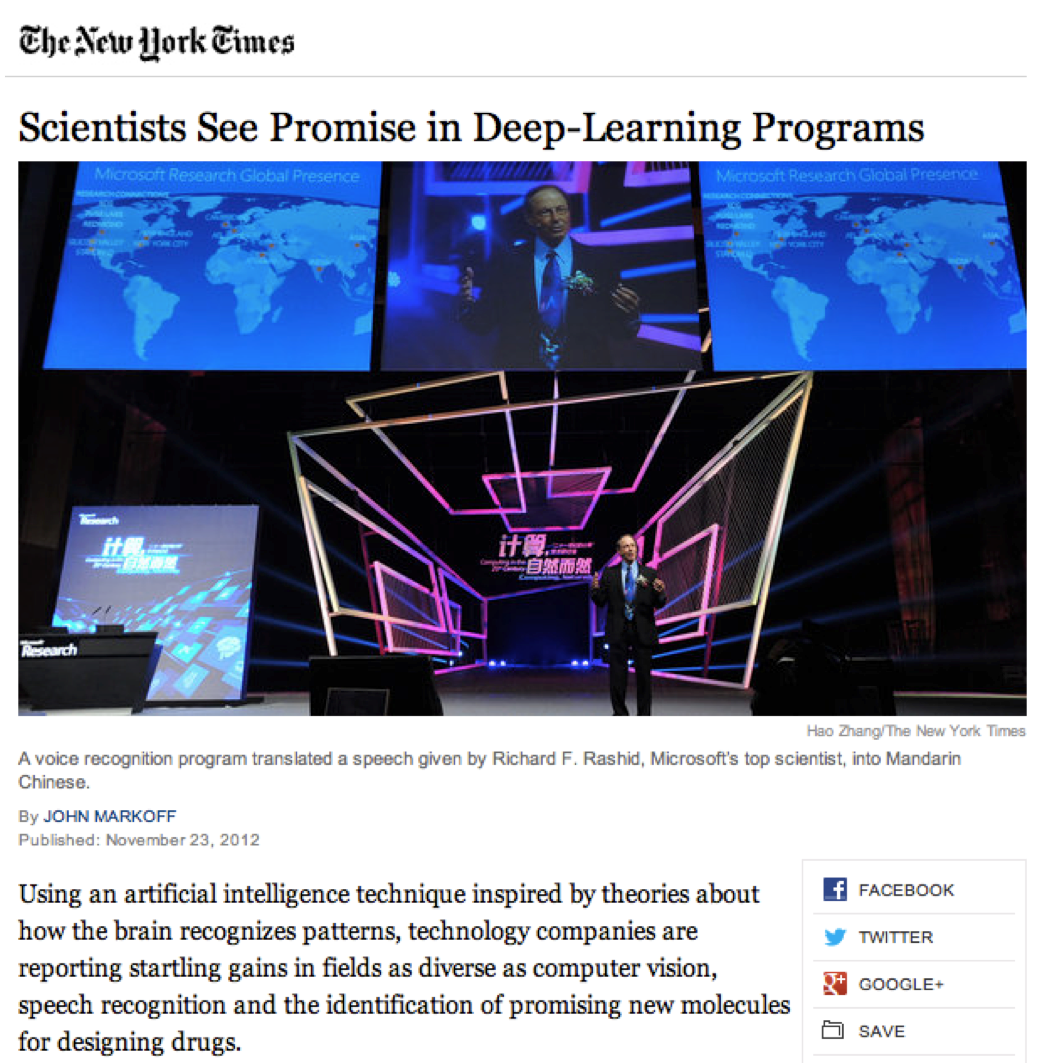
\includegraphics[scale=0.25]{figs/nyt_rashid}}
\end{frame}

%%%%%%%%%%%%%%%%
\begin{frame}
\centerline{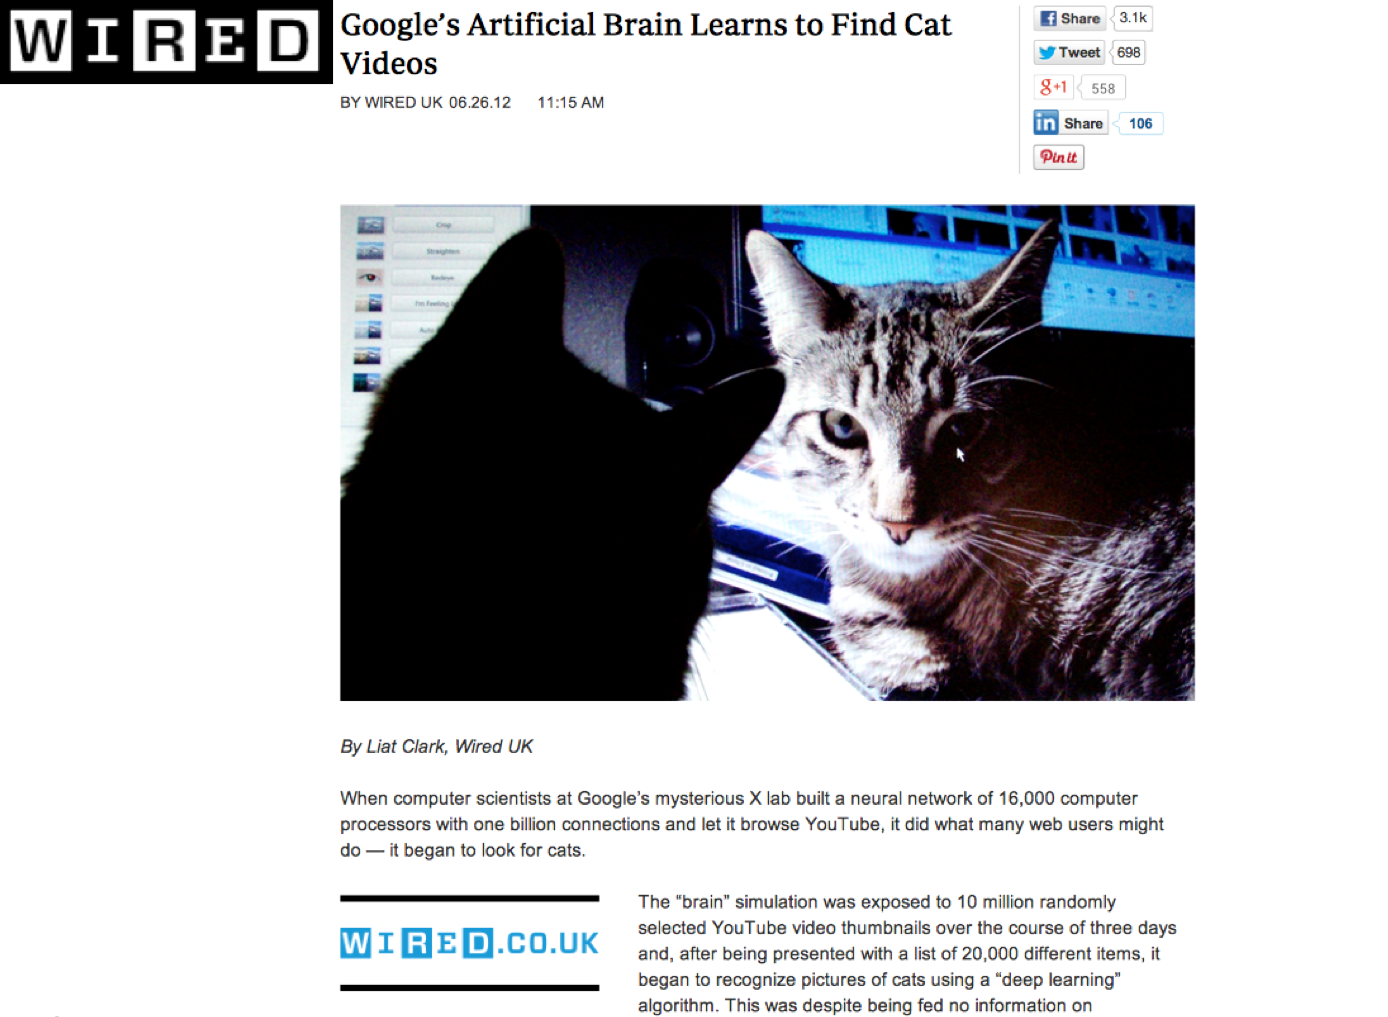
\includegraphics[scale=0.25]{figs/wired_googlecat}}
\end{frame}

%%%%%%%%%%%%%%%%
\begin{frame}
\centerline{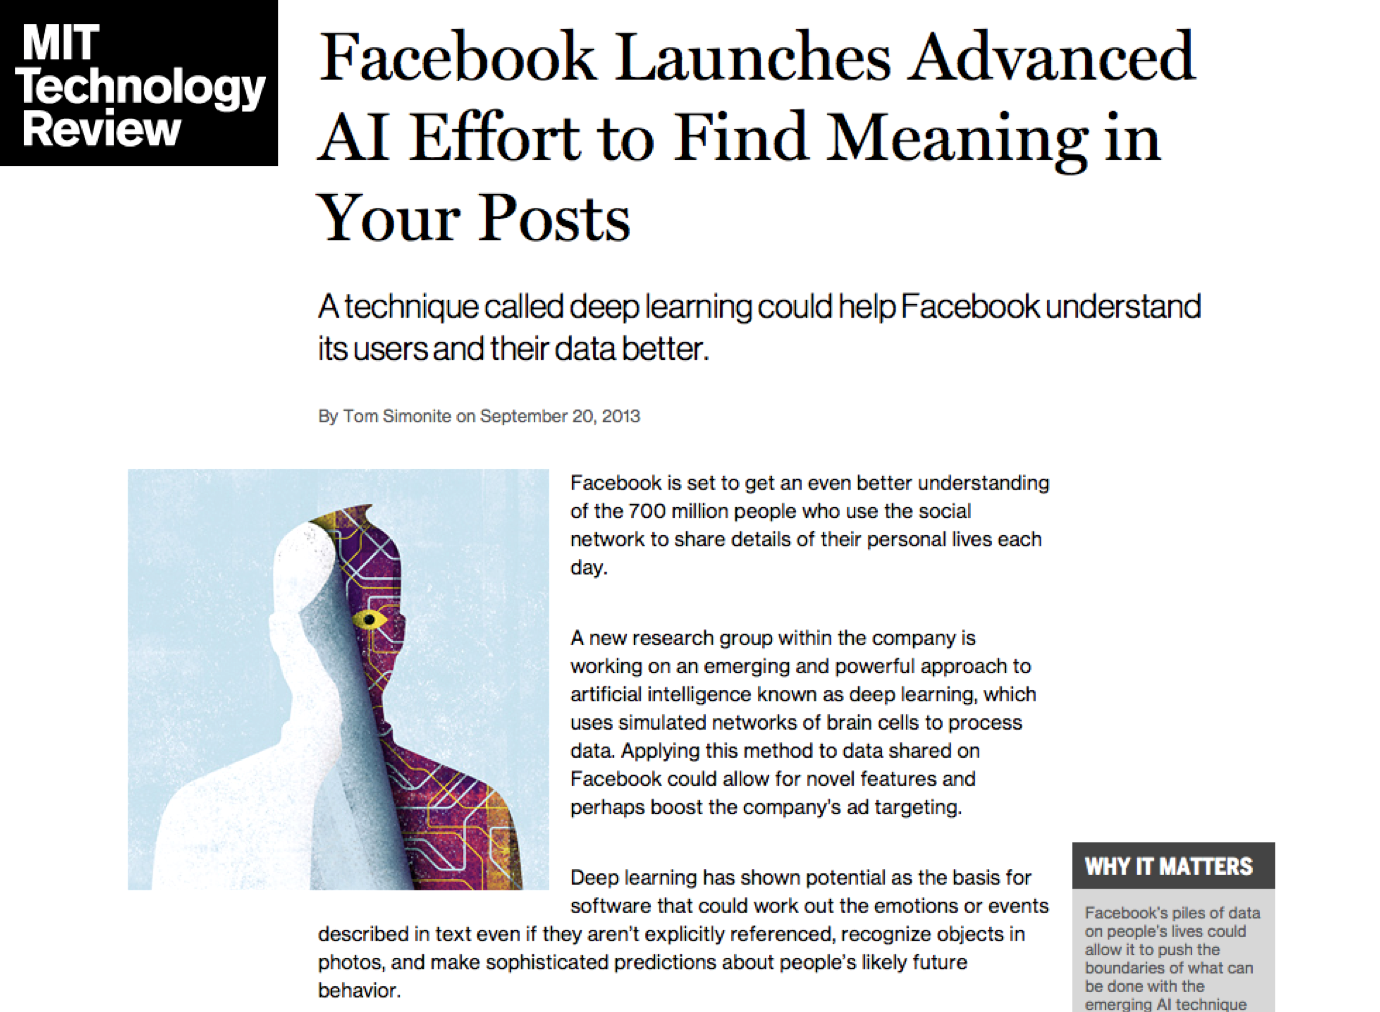
\includegraphics[scale=0.25]{figs/techreview_facebook}}
\end{frame}


%%%%%%%%%%%%%
\begin{frame}
\frametitle{What is Deep Learning?}
A family of methods that uses deep architectures to learn high-level feature representations
\pause
\centerline{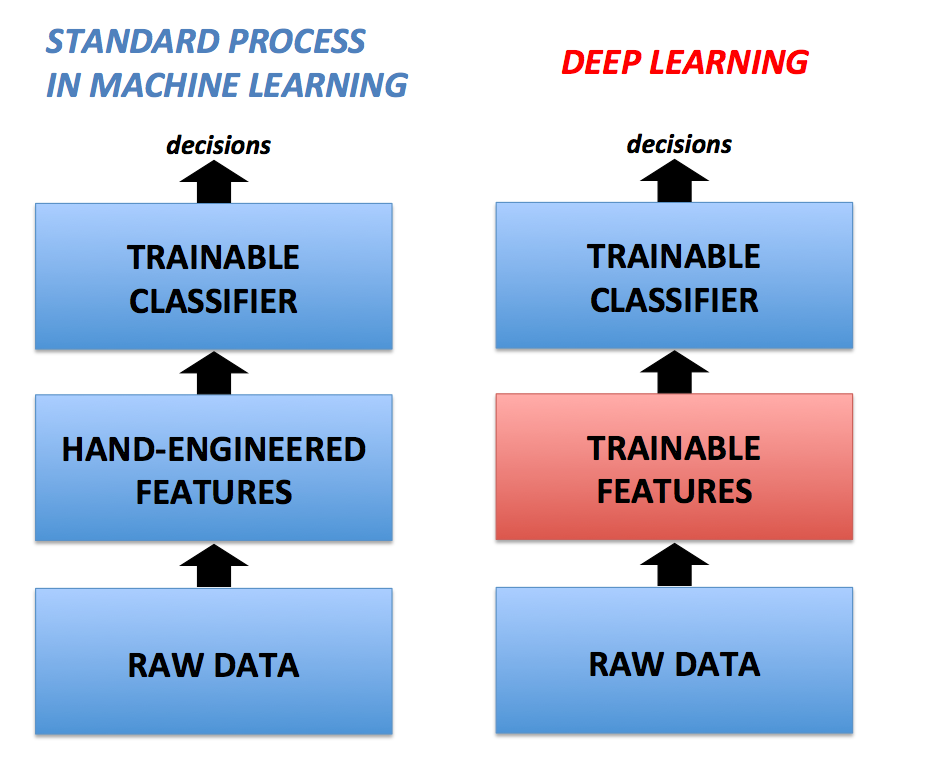
\includegraphics[scale=0.27]{figs/deep_vs_conventional_learning}}
\end{frame}

%%%%%%%%%%%%%
\begin{frame}
\frametitle{Example of Trainable Features }
Hierarchical object-parts features in Computer Vision \cite{lee09convolutional}
\centerline{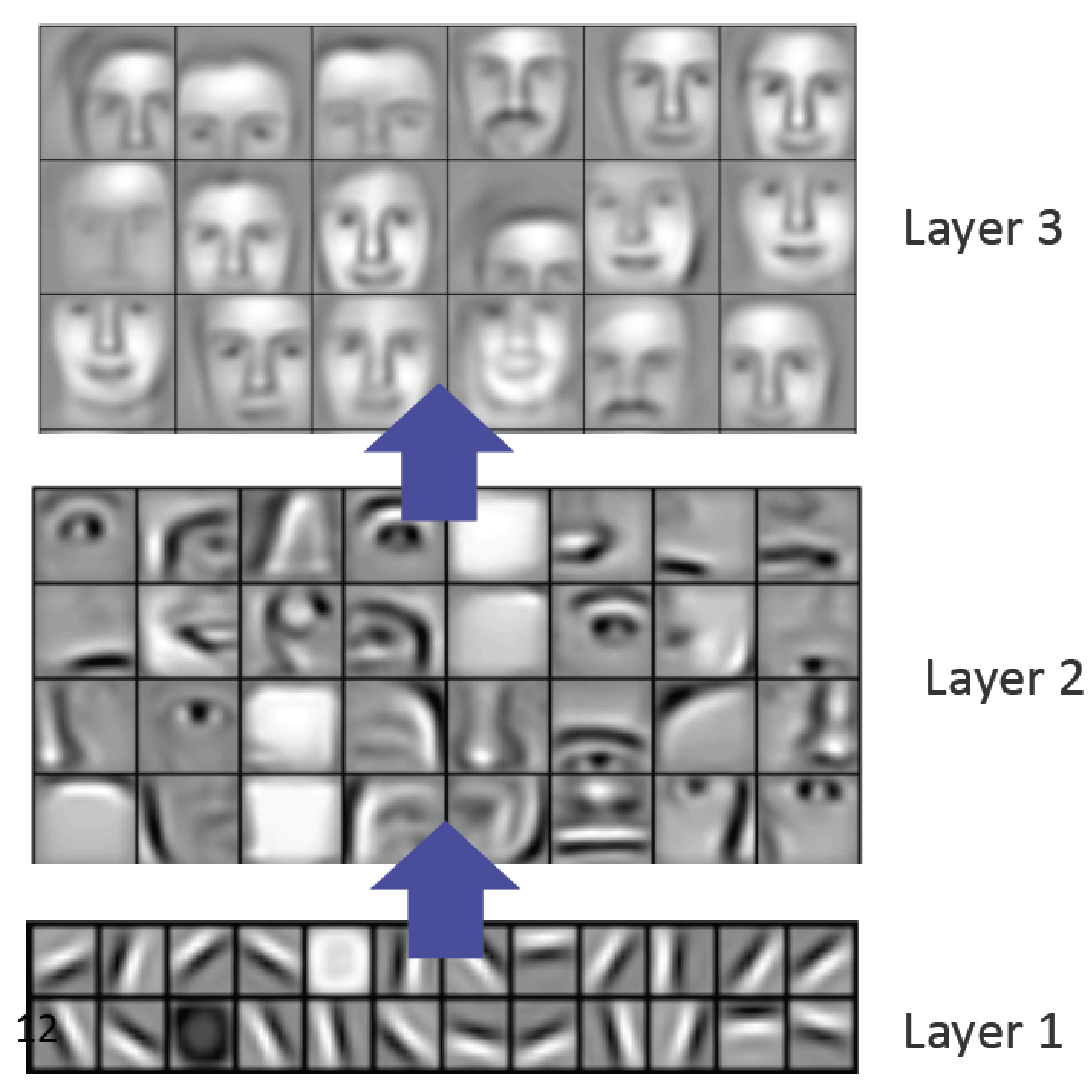
\includegraphics[scale=0.35]{figs/lee09example}}
\end{frame}


%%%%%%%%%%%%%
\begin{frame}
\frametitle{Course Outline}
\bi
\item Goal:\\To understand the foundations of neural networks and deep learning, at a level sufficient for reading recent research papers
\pause
\item Schedule: 
	\bi
	\item Lecture 1 (Jan 14): Machine Learning background \& Neural Networks
	\item Lecture 2 (Jan 16): Deep Architectures (DBN, SAE)
	\item Lecture 3 (Jan 21): Applications in Vision, Speech, Language
	\item Lecture 4 (Jan 23): Advanced topics in optimization
	\ei
\pause
\item Prerequisites: 
	\bi
	\item Basic calculus, probability, linear algebra
	\ei
\ei
\end{frame}

%%%%%%%%%%%%%
\begin{frame}
\frametitle{Course Material}
\bi
\item Course Website:\\ \url{http://cl.naist.jp/~kevinduh/a/deep2014/}
\vspace{0.5cm}
\item Useful References:
	\be
	\item Yoshua Bengio's \cite{bengio09book} short book: Learning Deep Architectures for AI\footnote{\url{http://www.iro.umontreal.ca/~bengioy/papers/ftml.pdf}}
	\item Yann LeCun \& Marc'Aurelio Ranzato's ICML2013 tutorial\footnote{\url{http://techtalks.tv/talks/deep-learning/58122/}}
	\item Richard Socher et.~al.'s NAACL2013 tutorial\footnote{\url{http://www.socher.org/index.php/DeepLearningTutorial/}}
	\item Geoff Hinton's Coursera course\footnote{\url{https://www.coursera.org/course/neuralnets}}
	\item Theano code samples\footnote{\url{http://deeplearning.net/tutorial/}}
	\item Chris Bishop's book Pattern Recognition and Machine Learning (PRML)\footnote{\url{http://research.microsoft.com/en-us/um/people/cmbishop/prml/}}
	\ee
\ei
\end{frame}

%%%%%%%%%%%%%
\begin{frame}
\frametitle{Grading}
\bi
\item The only criteria for grading:\\ Are you actively participating and asking questions in class?
	\bi
	\item If you ask (or answer) 3+ questions, grade = A
	\item If you ask (or answer) 2 questions, grade = B
	\item If you ask (or answer) 1 question, grade = C 
	\item If you don't ask (or answer) any questions, you get no credit.
	\ei
\ei
\end{frame}


%%%%%%%%%%%%%
\begin{frame}
\frametitle{Best Advice I got while in Grad School}
Always Ask Questions!
\bi
\pause
\item If you don't understand, you must ask questions in order to understand.
\pause
\item If you understand, you will naturally have questions. 
\pause
\item Having no questions is a sign that you are not thinking.
\ei
\end{frame}

%%%%%%%%%
\begin{frame}
\frametitle{Today's Topics}
\tableofcontents
\end{frame}

%SECTION%%%%%%%%%%%%%%%%%%%
\section{Machine Learning background}
%%%%%%%%%%%%%%%%%%%%

%% SUBSECTION%%%%%
\subsection[Why ML]{Why Machine Learning is needed?}

%%%%%%%%%%%%%
\begin{frame}
\frametitle{Write a Program$^*$\blfootnote{*example from Hinton's Coursera course} to Recognize the Digit 2}
This is hard to do manually!\\
\texttt{bool recognizeDigitAs2(int** imagePixels)\{...\}}
\centerline{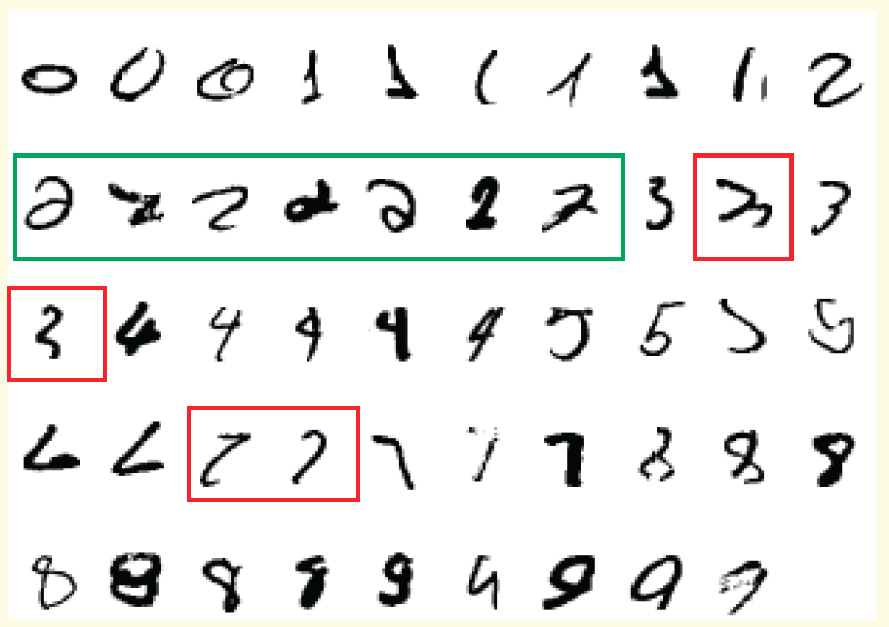
\includegraphics[scale=0.19]{figs/digit2}}\\
\pause
Machine Learning solution: 
\be
\item Assume you have a database (training data) of 2's and non-2's. 
\item Automatically "learn" this function from data
\ee
\end{frame}

%%%%%%%%%%%%%
\begin{frame}
\frametitle{A Machine Learning Solution}
Training data are represented as pixel matrices:
\begin{tikzpicture}
\draw[step=2mm,gray,very thin] (0,0) grid (2,2);
\fill[black](0.2,0.2) rectangle (1.8,0.4);
\fill[black](0.4,0.4) rectangle (0.6,0.6);
\fill[black](0.6,0.6) rectangle (0.8,0.8);
\fill[black](0.8,0.8) rectangle (1,1);
\fill[black](1,1) rectangle (1.2,1.2);
\fill[black](1.2,1.2) rectangle (1.4,1.4);
\fill[black](1.2,1.4) rectangle (1.4,1.6);
\fill[black](0.2,1.6) rectangle (1.4,1.8);
\end{tikzpicture}
\begin{tikzpicture}
\draw[step=2mm,gray,very thin] (0,0) grid (2,2);
\fill[black](1.2,0.2) rectangle (1.4,1.8);
\end{tikzpicture}
\vspace{5mm}
Classifier is parameterized by weight matrix of same dimension.\\
\pause
Training procedure: 
\be
\item When observe "2", add 1 to corresponding matrix elements
\item When observe "non-2", subtract 1 to corresponding matrix elements
\ee
\begin{center}
\scalebox{0.5}{\begin{tabular}{|c|c|c|c|c|c|c|c|c|c|}
\hline
0 & 0 & 0 & 0 & 0 & 0 & 0 & 0 & 0 & 0 \\
\hline
0 & 0 & 0 & 0 & 0 & 0 & 0 & 0 & 0 & 0 \\
\hline
0 & 0 & 0 & 0 & 0 & 0 & 0 & 0 & 0 & 0 \\
\hline
0 & 0 & 0 & 0 & 0 & 0 & 0 & 0 & 0 & 0 \\
\hline
0 & 0 & 0 & 0 & 0 & 0 & 0 & 0 & 0 & 0 \\
\hline
0 & 0 & 0 & 0 & 0 & 0 & 0 & 0 & 0 & 0 \\
\hline
0 & 0 & 0 & 0 & 0 & 0 & 0 & 0 & 0 & 0 \\
\hline
0 & 0 & 0 & 0 & 0 & 0 & 0 & 0 & 0 & 0 \\
\hline
0 & 0 & 0 & 0 & 0 & 0 & 0 & 0 & 0 & 0 \\
\hline
0 & 0 & 0 & 0 & 0 & 0 & 0 & 0 & 0 & 0 \\
\hline
\end{tabular}}
\begin{tikzpicture}
\draw[->,ultra thick] (0,0) to (0.4,0);
\end{tikzpicture}
\scalebox{0.5}{\begin{tabular}{|c|c|c|c|c|c|c|c|c|c|}
\hline
0 & 0 & 0 & 0 & 0 & 0 & 0 & 0 & 0 & 0 \\
\hline
0 & 1 & 1 & 1 & 1 & 1 & 1 & 0 & 0 & 0 \\
\hline
0 & 0 & 0 & 0 & 0 & 0 & 1 & 0 & 0 & 0 \\
\hline
0 & 0 & 0 & 0 & 0 & 0 & 1 & 0 & 0 & 0 \\
\hline
0 & 0 & 0 & 0 & 0 & 1 & 0 & 0 & 0 & 0 \\
\hline
0 & 0 & 0 & 0 & 1 & 0 & 0 & 0 & 0 & 0 \\
\hline
0 & 0 & 0 & 1 & 0 & 0 & 0 & 0 & 0 & 0 \\
\hline
0 & 0 & 1 & 0 & 0 & 0 & 0 & 0 & 0 & 0 \\
\hline
0 & 1 & 1 & 1 & 1 & 1 & 1 & 1 & 1 & 0 \\
\hline
0 & 0 & 0 & 0 & 0 & 0 & 0 & 0 & 0 & 0 \\
\hline
\end{tabular}}
\begin{tikzpicture}
\draw[->,ultra thick] (0,0) to (0.4,0);
\end{tikzpicture}
\scalebox{0.5}{\begin{tabular}{|c|c|c|c|c|c|c|c|c|c|}
\hline
0 & 0 & 0 & 0 & 0 & 0 & 0 & 0 & 0 & 0 \\
\hline
0 & 1 & 1 & 1 & 1 & 1 & 0 & 0 & 0 & 0 \\
\hline
0 & 0 & 0 & 0 & 0 & 0 & 0 & 0 & 0 & 0 \\
\hline
0 & 0 & 0 & 0 & 0 & 0 & 0 & 0 & 0 & 0 \\
\hline
0 & 0 & 0 & 0 & 0 & 1 & -1 & 0 & 0 & 0 \\
\hline
0 & 0 & 0 & 0 & 1 & 0 & -1 & 0 & 0 & 0 \\
\hline
0 & 0 & 0 & 1 & 0 & 0 & -1 & 0 & 0 & 0 \\
\hline
0 & 0 & 1 & 0 & 0 & 0 & -1 & 0 & 0 & 0 \\
\hline
0 & 1 & 1 & 1 & 1 & 1 & -1 & 1 & 1 & 0 \\
\hline
0 & 0 & 0 & 0 & 0 & 0 & 0 & 0 & 0 & 0 \\
\hline
\end{tabular}}
\end{center}
\pause
Test procedure: given new image, take sum of element-wise product.\\If positive, predict "2"; else predict "non-2".
\end{frame}

%% SUBSECTION%%%%%
\subsection[Main Concepts]{Main Concepts: Generalization, Model Expressiveness, Overfitting}


%%%%%%%%%%%%%
\begin{frame}
\frametitle{Generalization $\neq$ Memorization}
Key Issue in Machine Learning: Training data is limited
\bi
\item If the classifier just memorizes the training data, it may perform poorly on new data
\item "Generalization" is ability to extend accurate predictions to new data 
\ei
\pause
\vspace{1cm}
E.g. consider shifted image: \hspace{2cm} Will this classifier generalize?\\
\begin{tikzpicture}
\draw[step=2mm,gray,very thin] (0.2,0.2) grid (2.2,2.2);
\fill[black](0.2,0.2) rectangle (1.8,0.4);
\fill[black](0.4,0.4) rectangle (0.6,0.6);
\fill[black](0.6,0.6) rectangle (0.8,0.8);
\fill[black](0.8,0.8) rectangle (1,1);
\fill[black](1,1) rectangle (1.2,1.2);
\fill[black](1.2,1.2) rectangle (1.4,1.4);
\fill[black](1.2,1.4) rectangle (1.4,1.6);
\fill[black](0.2,1.6) rectangle (1.4,1.8);
\end{tikzpicture}
\begin{tikzpicture}
\draw[step=2mm,gray,very thin] (0,-0.2) grid (2,1.8);
\fill[black](0.2,0.2) rectangle (1.8,0.4);
\fill[black](0.4,0.4) rectangle (0.6,0.6);
\fill[black](0.6,0.6) rectangle (0.8,0.8);
\fill[black](0.8,0.8) rectangle (1,1);
\fill[black](1,1) rectangle (1.2,1.2);
\fill[black](1.2,1.2) rectangle (1.4,1.4);
\fill[black](1.2,1.4) rectangle (1.4,1.6);
\fill[black](0.2,1.6) rectangle (1.4,1.8);
\end{tikzpicture}
\begin{tikzpicture}
\draw[step=2mm,gray,very thin] (0,0) grid (2,2);
\fill[black](0.2,0.2) rectangle (1.8,0.4);
\fill[black](0.4,0.4) rectangle (0.6,0.6);
\fill[black](0.6,0.6) rectangle (0.8,0.8);
\fill[black](0.8,0.8) rectangle (1,1);
\fill[black](1,1) rectangle (1.2,1.2);
\fill[black](1.2,1.2) rectangle (1.4,1.4);
\fill[black](1.2,1.4) rectangle (1.4,1.6);
\fill[black](0.2,1.6) rectangle (1.4,1.8);
\end{tikzpicture}
\hspace{1.5cm}
\scalebox{0.5}{\begin{tabular}{|c|c|c|c|c|c|c|c|c|c|}
\hline
0 & 0 & 0 & 0 & 0 & 0 & 0 & 0 & 0 & 0 \\
\hline
0 & 1 & 1 & 1 & 1 & 1 & 0 & 0 & 0 & 0 \\
\hline
0 & 0 & 0 & 0 & 0 & 0 & 0 & 0 & 0 & 0 \\
\hline
0 & 0 & 0 & 0 & 0 & 0 & 0 & 0 & 0 & 0 \\
\hline
0 & 0 & 0 & 0 & 0 & 1 & -1 & 0 & 0 & 0 \\
\hline
0 & 0 & 0 & 0 & 1 & 0 & -1 & 0 & 0 & 0 \\
\hline
0 & 0 & 0 & 1 & 0 & 0 & -1 & 0 & 0 & 0 \\
\hline
0 & 0 & 1 & 0 & 0 & 0 & -1 & 0 & 0 & 0 \\
\hline
0 & 1 & 1 & 1 & 1 & 1 & -1 & 1 & 1 & 0 \\
\hline
0 & 0 & 0 & 0 & 0 & 0 & 0 & 0 & 0 & 0 \\
\hline
\end{tabular}}
\end{frame}

%%%%%%%%%%%%%
\begin{frame}
\frametitle{Generalization $\neq$ Memorization}
One potential way to increase generalization ability:
\bi
\item Discretize weight matrix with larger grids (fewer weights to train)
\ei
E.g. consider shifted image:\\
\begin{tikzpicture}
\draw[step=2mm,gray,very thin] (0.2,0.2) grid (2.2,2.2);
\fill[black](0.2,0.2) rectangle (1.8,0.4);
\fill[black](0.4,0.4) rectangle (0.6,0.6);
\fill[black](0.6,0.6) rectangle (0.8,0.8);
\fill[black](0.8,0.8) rectangle (1,1);
\fill[black](1,1) rectangle (1.2,1.2);
\fill[black](1.2,1.2) rectangle (1.4,1.4);
\fill[black](1.2,1.4) rectangle (1.4,1.6);
\fill[black](0.2,1.6) rectangle (1.4,1.8);
\end{tikzpicture}
\begin{tikzpicture}
\draw[step=2mm,gray,very thin] (0,-0.2) grid (2,1.8);
\fill[black](0.2,0.2) rectangle (1.8,0.4);
\fill[black](0.4,0.4) rectangle (0.6,0.6);
\fill[black](0.6,0.6) rectangle (0.8,0.8);
\fill[black](0.8,0.8) rectangle (1,1);
\fill[black](1,1) rectangle (1.2,1.2);
\fill[black](1.2,1.2) rectangle (1.4,1.4);
\fill[black](1.2,1.4) rectangle (1.4,1.6);
\fill[black](0.2,1.6) rectangle (1.4,1.8);
\end{tikzpicture}
\begin{tikzpicture}
\draw[step=4mm,gray,very thin] (0,0) grid (2,2);
\fill[black](0.2,0.2) rectangle (1.8,0.4);
\fill[black](0.4,0.4) rectangle (0.6,0.6);
\fill[black](0.6,0.6) rectangle (0.8,0.8);
\fill[black](0.8,0.8) rectangle (1,1);
\fill[black](1,1) rectangle (1.2,1.2);
\fill[black](1.2,1.2) rectangle (1.4,1.4);
\fill[black](1.2,1.4) rectangle (1.4,1.6);
\fill[black](0.2,1.6) rectangle (1.4,1.8);
\end{tikzpicture}

Now will this classifier generalize?\\
\scalebox{0.5}{\begin{tabular}{|c|c|c|c|c|c|c|c|c|c|}
\hline
0 & 0 & 0 & 0 & 0 & 0 & 0 & 0 & 0 & 0 \\
\hline
0 & 1 & 1 & 1 & 1 & 1 & 0 & 0 & 0 & 0 \\
\hline
0 & 0 & 0 & 0 & 0 & 0 & 0 & 0 & 0 & 0 \\
\hline
0 & 0 & 0 & 0 & 0 & 0 & 0 & 0 & 0 & 0 \\
\hline
0 & 0 & 0 & 0 & 0 & 1 & -1 & 0 & 0 & 0 \\
\hline
0 & 0 & 0 & 0 & 1 & 0 & -1 & 0 & 0 & 0 \\
\hline
0 & 0 & 0 & 1 & 0 & 0 & -1 & 0 & 0 & 0 \\
\hline
0 & 0 & 1 & 0 & 0 & 0 & -1 & 0 & 0 & 0 \\
\hline
0 & 1 & 1 & 1 & 1 & 1 & -1 & 1 & 1 & 0 \\
\hline
0 & 0 & 0 & 0 & 0 & 0 & 0 & 0 & 0 & 0 \\
\hline
\end{tabular}}
\begin{tikzpicture}
\draw[->,ultra thick] (0,0) to (0.4,0);
\end{tikzpicture}
\scalebox{0.485}{\begin{tabular}{|c|c||c|c||c|c||c|c||c|c|}
\hline
0 & 0 & 0 & 0 & 0 & 0 & 0 & 0 & 0 & 0 \\
\hline
0 & 1 & 1 & 1 & 1 & 1 & 0 & 0 & 0 & 0 \\
\hline\hline
0 & 0 & 0 & 0 & 0 & 0 & 0 & 0 & 0 & 0 \\
\hline
0 & 0 & 0 & 0 & 0 & 0 & 0 & 0 & 0 & 0 \\
\hline\hline
0 & 0 & 0 & 0 & 0 & 1 & -1 & 0 & 0 & 0 \\
\hline
0 & 0 & 0 & 0 & 1 & 0 & -1 & 0 & 0 & 0 \\
\hline\hline
0 & 0 & 0 & 1 & 0 & 0 & -1 & 0 & 0 & 0 \\
\hline
0 & 0 & 1 & 0 & 0 & 0 & -1 & 0 & 0 & 0 \\
\hline\hline
0 & 1 & 1 & 1 & 1 & 1 & -1 & 1 & 1 & 0 \\
\hline
0 & 0 & 0 & 0 & 0 & 0 & 0 & 0 & 0 & 0 \\
\hline
\end{tabular}}
\begin{tikzpicture}
\draw[->,ultra thick] (0,0) to (0.4,0);
\end{tikzpicture}
\scalebox{1}{\begin{tabular}{|c|c|c|c|c|}
\hline
1 & 1 & 1 & 0 & 0 \\ \hline
0 & 0 & 0 & 0 & 0 \\ \hline
0 & 0 & 1 & -1 & 0 \\ \hline
0 & 1 & 0 & -1 & 0 \\ \hline
1 & 1 & 1 & 0  & 1 \\ \hline
\end{tabular}}
\end{frame}



%%%%%%%%%%%%%
\begin{frame}
\frametitle{Model Expressiveness and Overfitting}
\bi
\item A model with more weight parameters may fit training data better
\item But since training data is limited, expressive model stand the risk of overfitting to peculiarities of the data.
\ei
\begin{center}
Less Expressive Model $\Longleftrightarrow$ More Expressive Model \\
(fewer weights) \hspace{1cm} (more weights) \\[0.5cm]
Underfit training data $\Longleftrightarrow$ Overfit training data \\
\end{center}
\end{frame}

%%%%%%%%%%%%%
\begin{frame}
\frametitle{Model Expressiveness and Overfitting}
Fitting the training data (blue points: $x_n$)\\
with a polynomial model: $f(x)=w_0 + w_1x + w_2x^2 + \ldots + w_Mx^M$\\
under squared error objective $\frac{1}{2} \sum_n (f(x_n) - t_n)^2$

\blfootnote{from PRML Chapter 1 \cite{bishopPRML}}

\begin{center}
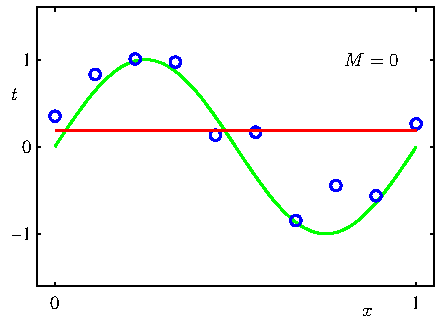
\includegraphics[scale=0.55]{figs/polyfit_a}
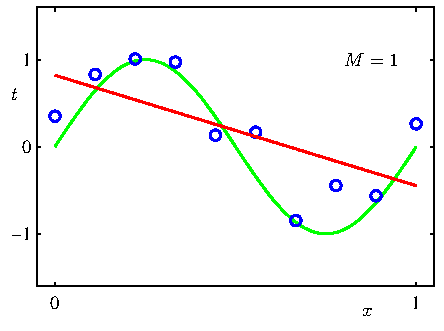
\includegraphics[scale=0.55]{figs/polyfit_b}\\
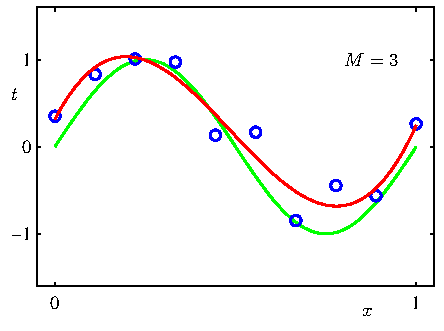
\includegraphics[scale=0.55]{figs/polyfit_c}
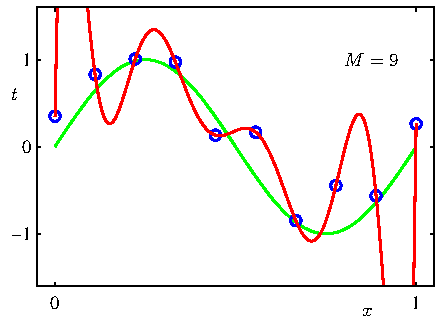
\includegraphics[scale=0.55]{figs/polyfit_d}
\end{center}
\end{frame}



%% SUBSECTION%%%%%
\subsection[Notation]{Formal Notation}

%%%%%%%%%%%%%
\begin{frame}
\frametitle{Basic Problem Setup in Machine Learning}
\bi
\item Training Data: a set of $(x^{(m)},y^{(m)})_{m=\{1,2,..M\}}$ pairs, where input $x^{(m)} \in R^d$ and output $y^{(m)}=\{0,1\}$ 
	\bi
	\item e.g. x=vectorized image pixels, y=2 or non-2
	\ei
\item Goal: Learn function $f: x \rightarrow y$ to predicts correctly on new inputs $x$.
\pause
\bi
\item Step 1: Choose a function model family:
	\bi
	\item e.g. logistic regression, support vector machines, neural networks
	\ei
\pause
\item Step 2: Optimize parameters $w$ on the Training Data
	\bi 
	\item e.g. minimize loss function $\min_{w} \sum_{m=1}^M  ( f_w(x^{(m)}) - y^{(m)} )^2$
	\ei
\ei
\ei
\end{frame}

%%%%%%%%%%%%%
%\begin{frame}
%\frametitle{No Free Lunch}
%\bi
%\item No machine learning method is best for all datasets 
%\item You must learn to choose an appropriate model family and optimization algorithm for your task
%\ei
%\end{frame}


%SECTION%%%%%%%%%%%%%%%%%%%
\section{Neural Networks}
%%%%%%%%%%%%%%%%%%%%


%% SUBSECTION%%%%%
\subsection[1-Layer Nets]{1-Layer Nets (Logistic Regression)}

%%%%%%%%%%%%%
\begin{frame}
\frametitle{1-Layer Nets (Logistic Regression)}
\bi
\item Function model: $f(x)=\sigma(w^T \cdot x + b)$
	\bi
	\item Parameters: vector $w \in R^d$, $b$ is scalar bias term
	\item $\sigma$ is a non-linearity, e.g. sigmoid: $\sigma(z) = 1/(1+\exp(-z))$
	\item For simplicity, sometimes write $f(x)=\sigma(w^T x)$ where $w=[w;b]$ and $x=[x;1]$
	\ei
\centerline{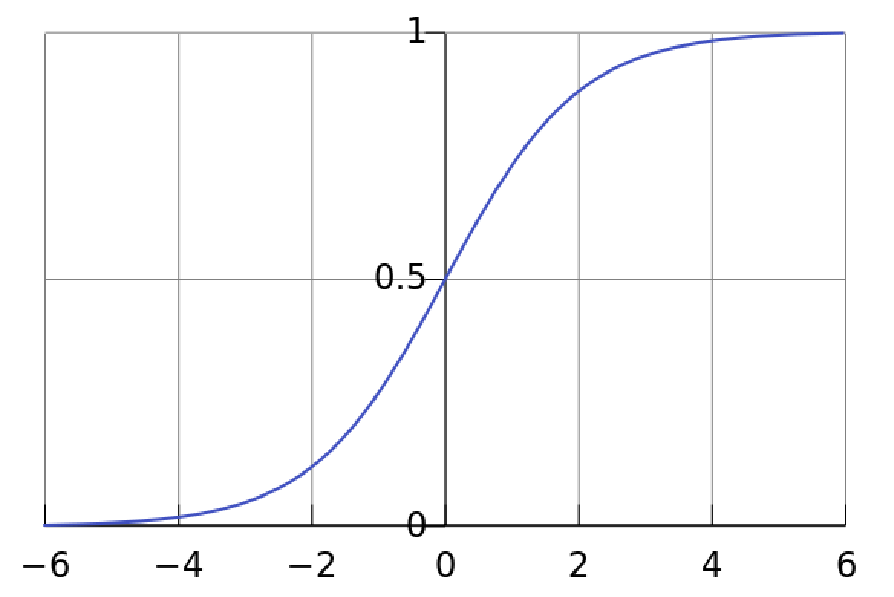
\includegraphics[scale=0.3]{figs/sigmoid}}
\pause
\item Non-linearity will be important in expressiveness multi-layer nets. Other non-linearities, e.g., $tanh(z)=(e^z-e^{-z}) / (e^z+e^{-z})$
\ei
\end{frame}


%%%%%%%%%%%%%
\begin{frame}
\frametitle{Training 1-Layer Nets: Gradient}
\bi
\item Assume Squared-Error$^*$ $Loss(w) = \frac{1}{2} \sum_{m}  ( \sigma(w^T x^{(m)}) - y^{(m)} )^2$
\pause
%\item Gradient: $\nabla_w Loss = \sum_m {\color{red} ( \sigma(w^T x^{(m)}) - y^{(m)} )} {\color{blue} (\sigma(w^Tx^{(m)}) (1- \sigma(w^Tx^{(m)}) )} x^{(m)}$
\item Gradient: $\nabla_w Loss = \sum_m {\color{red} \left[ \sigma(w^T x^{(m)}) - y^{(m)} \right]} {\color{blue} \sigma'(w^Tx^{(m)})} x^{(m)}$
	\bi
	\pause
	\item General form of gradient: $\sum_m{\color{red} Error^{(m)}} * {\color{blue} \sigma'(in^{(m)})} * x^{(m)}$
	\ei
\pause
\item Derivative of sigmoid $\sigma(z) = 1/(1+\exp(-z))$:
	\begin{columns}
		\begin{column}{0.4\textwidth}
		\begin{small}
		\begin{eqnarray*}
				\sigma'(z)	& = &  \frac{d}{dz}\left(\frac{1}{1+\exp(-z)}\right) \\
						& = &  -\left(\frac{1}{1+\exp(-z)}\right)^2 \frac{d}{dz}(1+\exp(-z))\\
						& =  & -\left(\frac{1}{1+\exp(-z)}\right)^2 \exp(-z)(-1)\\
						& =  & \left(\frac{1}{1+\exp(-z)}\right) \left(\frac{\exp(-z)}{1+\exp(-z)}\right)  \\
						& = & \sigma(z) (1-\sigma(z))
		\end{eqnarray*}
		\end{small}
		\end{column}
		\begin{column}{0.5\textwidth}
	\hfill		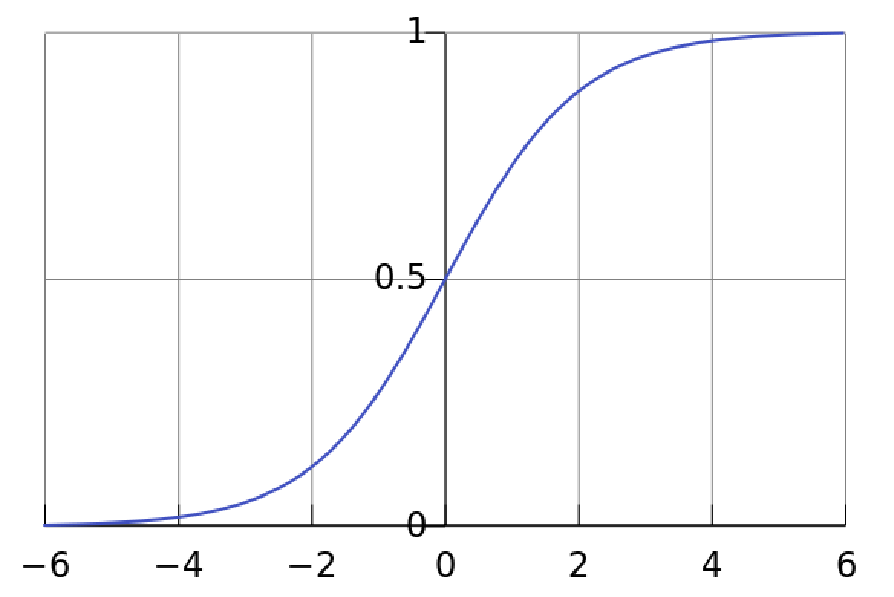
\includegraphics[scale=0.25]{figs/sigmoid}
		\end{column}
		
	\end{columns}
\ei
\vspace{-0.8cm}
\blfootnote{\hspace{-0.4cm}*An alternative is Cross-Entropy loss: $\sum_m~y^{(m)} \log(\sigma(w^Tx^{(m)}))+(1-y^{(m)}) \log(1-\sigma(w^Tx^{(m)}))$ }

\end{frame}

%%%%%%%%%%%%%
\begin{frame}
\frametitle{Training 1-Layer Nets: Gradient Descent Algorithm}
\bi
\item General form of gradient: $\sum_m{\color{red} Error^{(m)}} * {\color{blue} \sigma'(in^{(m)})} * x^{(m)}$
\item Gradient descent algorithm:
	\be
	\item Initialize $w$
	%\item Compute $\nabla_w Loss = \sum_m{\color{red} (\sigma(w^Tx^{(m)})-y^{(m)})} * {\color{blue} \sigma'(w^Tx^{(m)})} * x^{(m)}$
	\item Compute $\nabla_w Loss = \sum_m{\color{red} Error^{(m)}} * {\color{blue} \sigma'(in^{(m)})} * x^{(m)}$
	\item $w \leftarrow w - \gamma( \nabla_w Loss )$
	\item Repeat steps 2-3 until some condition satisfied 
	\ee
\pause
\item Stochastic gradient descent (SGD) algorithm:
	\be
	\item Initialize $w$
	\item for each sample $(x^{(m)},y^{(m)})$ in training set:
	%\item \hspace{1cm} $w \leftarrow w - \gamma({\color{red} (\sigma(w^Tx^{(m)})-y^{(m)})} * {\color{blue} \sigma'(w^Tx^{(m)})} * x^{(m)} )$
	\item \hspace{1cm} $w \leftarrow w - \gamma({\color{red} Error^{(m)}} * {\color{blue} \sigma'(in^{(m)})} * x^{(m)})$
	\item Repeat loop 2-3 until some condition satisfied 
	\ee
\pause
\item Learning rate $\gamma>0$  \& stopping condition are important in practice
\ei
\end{frame}

%%%%%%%%%%%%%
\begin{frame}
\frametitle{Intuition of SGD update}
\bi
\item for some sample $(x^{(m)},y^{(m)})$:\\
 \hspace{1cm} $w \leftarrow w - \gamma({\color{red} (\sigma(w^Tx^{(m)})-y^{(m)})} * {\color{blue} \sigma'(w^Tx^{(m)})} * x^{(m)} )$
\ei
\begin{center}
\begin{tabular}{|c|c|c|c|c|}
\hline
$\sigma(w^Tx^{(m)})$ & $y^{(m)}$ & ${\color{red}Error}$ & new w & new prediction \\\hline\hline
0 & 0 & 0 & no change & 0 \\\hline
1 & 1 & 0 & no change & 1 \\\hline
0 & 1 & -1 & $w + \gamma \sigma'(in^{(m)})x^{(m)}$ & $\geq0$ \\\hline
1 & 0 & +1 & $w - \gamma \sigma'(in^{(m)})x^{(m)}$ & $\leq1$ \\\hline
\end{tabular}
\end{center}
\pause
\bi
\item \begin{small} $\left[w + \gamma \sigma'(in^{(m)})x^{(m)}\right]^T x^{(m)} = w^Tx^{(m)} + \gamma \sigma'(in^{(m)})||x^{(m)}||^2  \geq w^Tx^{(m)} $ \end{small}
\pause
\item $\sigma'(w^Tx^{(m)})$ is near 0 when confident, near 0.25 when uncertain.
\pause
\item large $\gamma$ = more aggressive updates; small $\gamma$ = more conservative
\pause
\item SGD improves classification for current sample, but no guarantee about others
\ei
\end{frame}

%%%%%%%%%%%%%
\begin{frame}
\frametitle{Geometric view of SGD update}
\bi
\item Loss objective contour plot: \begin{small}$\frac{1}{2} \sum_{m}  ( \sigma(w^T x^{(m)}) - y^{(m)} )^2 + ||w||$\end{small}
\bi
	\item Gradient descent goes in steepest descent direction, but slower to compute per iteration for large datasets
	\item SGD can be viewed as noisy descent, but faster per iteration
	\item In practice, a good tradeoff is mini-batch SGD
\ei
\ei
\centerline{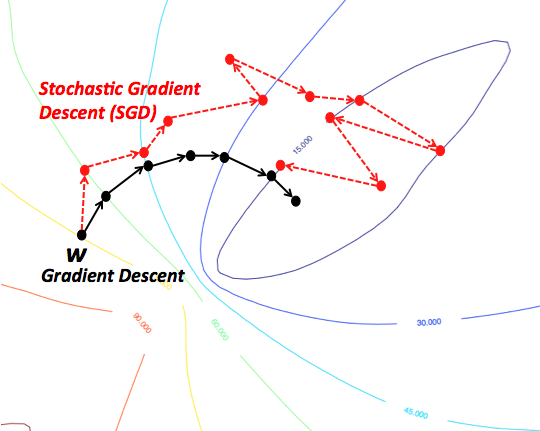
\includegraphics[scale=0.4]{figs/sgd_contour}}
\end{frame}

%%%%%%%%%%%%%
\begin{frame}
\frametitle{Effect of Learning Rate $\gamma$ on Convergence Speed}
\bi
\item SGD update: $w \leftarrow w - \gamma({\color{red} Error^{(m)}} * {\color{blue} \sigma'(in^{(m)})} * x^{(m)})$
\bi
	\item Ideally, $\gamma$ should be as large as possible without causing divergence.
	\item Common heuristic: $\gamma(t) = \frac{\gamma_0}{1+\nu t} = O(1/t)$ 
\ei
\item Analysis by \cite{schaul13learningrate} (in plot, $\eta \equiv \gamma$):
\ei
\centerline{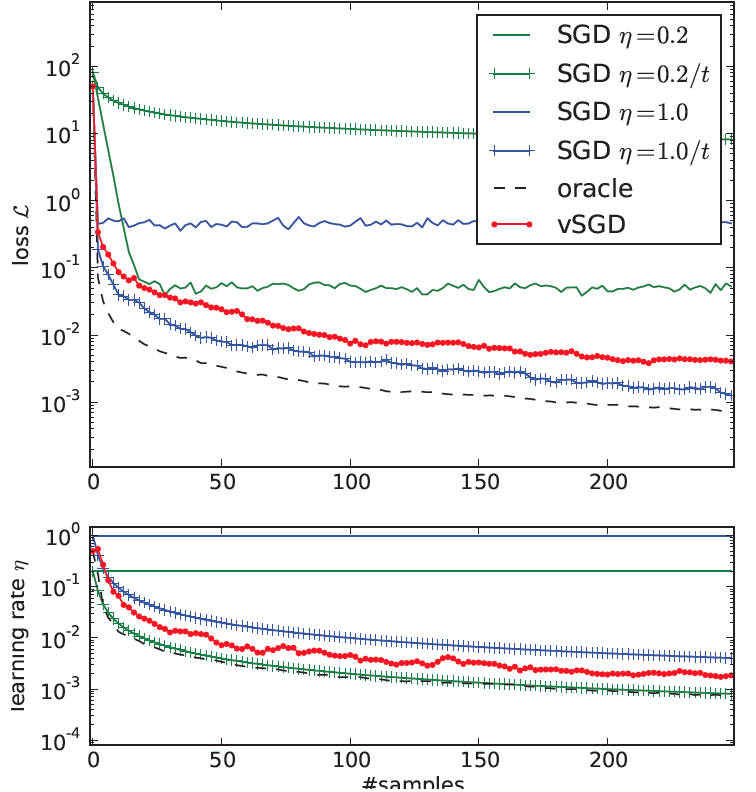
\includegraphics[scale=0.23]{figs/schaul13learningrate}}
\end{frame}


%%%%%%%%%%%%%
\begin{frame}
\frametitle{Generalization issues: Regularization and Early-stopping}
\bi
\item Optimizing $Loss(w) = \frac{1}{2} \sum_{m}  ( \sigma(w^T x^{(m)}) - y^{(m)} )^2$ on training data not necessarily leads to generalization. 
\pause
\be
	\item Adding regularization:  $Loss(w) = \frac{1}{2} \sum_{m}  ( \sigma(w^T x^{(m)}) - y^{(m)} )^2 + ||w||$ reduces sensitivity to training input and decreases risk of overfitting
	\pause
	\item Early Stopping:
	\bi
	\item Prepare separate training and validation (development) data
	\item Optimize $Loss(w)$ on training but stop when $Loss(w)$ on validation stops improving 
	\ei
\ee
\ei
\begin{center}
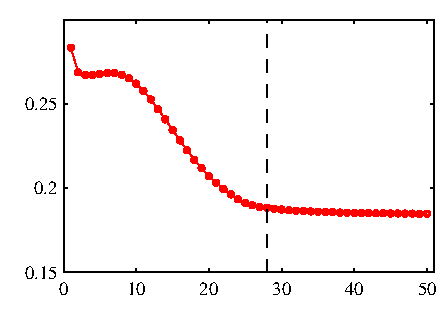
\includegraphics[scale=0.7]{figs/earlystop_a}
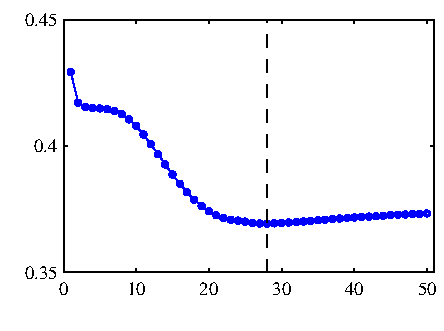
\includegraphics[scale=0.7]{figs/earlystop_b}
\end{center}
\blfootnote{Figures from Chapter 5, \cite{bishopPRML}}
\end{frame}

%%%%%%%%%%%%%
\begin{frame}
\frametitle{Summary}
\be
\item Given Training Data: $(x^{(m)},y^{(m)})_{m=\{1,2,..M\}}$
\item Optimize a model $f(x)=\sigma(w^T \cdot x + b)$ under $Loss(w) = \frac{1}{2} \sum_{m}  ( \sigma(w^T x^{(m)}) - y^{(m)} )^2$
\pause
\item General form of gradient: $\sum_m{\color{red} Error^{(m)}} * {\color{blue} \sigma'(in^{(m)})} * x^{(m)}$
\pause
\item SGD algorithm: for each sample $(x^{(m)},y^{(m)})$ in training set,\\
	\hspace{1cm} $w \leftarrow w - \gamma({\color{red} Error^{(m)}} * {\color{blue} \sigma'(in^{(m)})} * x^{(m)})$
\pause
\item Important issues: 
	\bi
	\item Optimization speed/convergence: batch vs. mini-batch, learning rate $\gamma$
	\item Generalization ability: regularization, early-stopping
	\ei
\ee
\end{frame}

%% SUBSECTION%%%%%
\subsection[Expressiveness]{2-Layer Nets and Model Expressiveness}

%%%%%%%%%%%%%
\begin{frame}
\frametitle{2-Layer Neural Networks}
\begin{tikzpicture}[->,>=stealth',shorten >=1pt,auto,node distance=3cm,
  thick,main node/.style={circle,fill=blue!20,draw,font=\sffamily\Large\bfseries}]

  \node[main node] (1) at (1,0) {$x_1$};
  \node[main node] (2) at (3,0) {$x_2$};
  \node[main node] (3) at (5,0) {$x_3$};
  \node[main node] (4) at (7,0) {$x_4$};
  \node[main node] (h1) at (2,2) {$h_1$};
  \node[main node] (h2) at (4,2) {$h_2$};
  \node[main node] (h3) at (6,2) {$h_3$};
  \node[main node] (y) at (4,4) {$y$};

   \node(xi) at (0,0) {$x_i$};
   \node(wij) at (0,1) {$w_{ij}$};
   \node(hj) at (0,2) {$h_j$};
   \node(wj) at (0,3) {$w_{j}$};

	

  \path[every node/.style={font=\sffamily\small}]
    (1) edge node [left] {$w_{11}$} (h1)
    (2) edge node {} (h1)
    (3) edge node {} (h1)
    (4) edge node {} (h1)
    (1) edge node [left] {$w_{12}$} (h2)
    (2) edge node {} (h2)
    (3) edge node {} (h2)
    (4) edge node {} (h2)
    (1) edge node {} (h3)
    (2) edge node {} (h3)
    (3) edge node {} (h3)
    (4) edge node {} (h3)
    (h1) edge node [left] {$w_1$} (y)
    (h2) edge node [left] {$w_2$} (y)
    (h3) edge node [left] {$w_3$} (y)
    ;
\end{tikzpicture}

\vspace{4mm}
\begin{math}
f(x)=\sigma(\sum_j w_j \cdot h_j)
= \sigma(\sum_j w_j \cdot \sigma(\sum_i w_{ij}  x_i))
\end{math}\\
\pause
\vspace{0.3cm}
Hidden units $h_j$'s can be viewed as new "features" from combining $x_i$'s
\blfootnote{\hspace{-0.5cm}Called Multilayer Perceptron (MLP), but more like multilayer logistic regression}
\end{frame}


%%%%%%%%%%%%%%%%
\begin{frame}
\frametitle{Modeling complex non-linearities}
\bi
\item Given same number of units (with non-linear activation), a deeper architecture is more expressive than a shallow one
\cite{bishop95book}
\bi
	\item 1-layer nets only model linear hyperplanes
	\item 2-layer nets are universal function approximators: given infinite hidden nodes, it can express any continuous function
	\item $>$3-layer nets can do so with fewer nodes/weights
\ei
\ei
\centerline{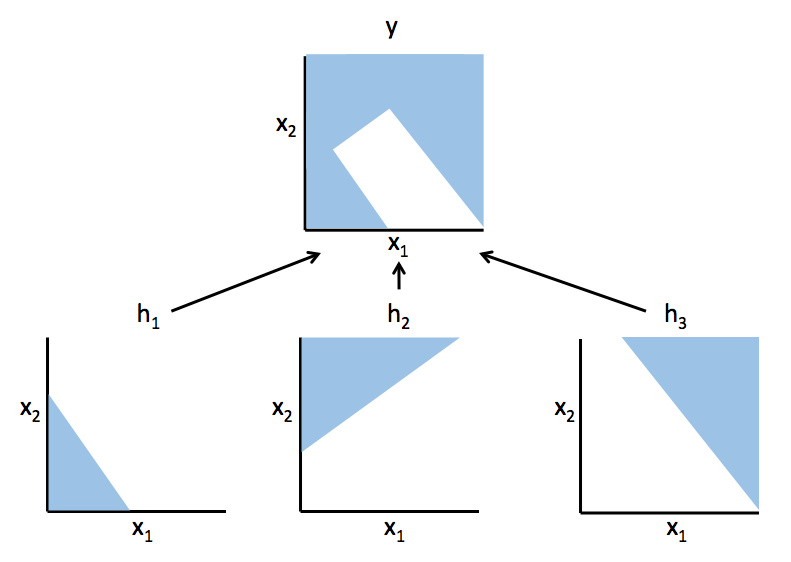
\includegraphics[scale=0.27]{figs/twolayer_nonlinearity}}
\end{frame}


%% SUBSECTION%%%%%
\subsection[Backpropagation]{Training by Backpropagation}


%%%%%%%%%%%%%
\begin{frame}
\frametitle{Training a 2-Layer Net with Backpropagation}
\begin{tikzpicture}[->,>=stealth',shorten >=1pt,auto,node distance=3cm,
  thick,main node/.style={circle,fill=blue!20,draw,font=\sffamily\Large\bfseries}]

  \node[main node] (1) at (1,0) {$x_1$};
  \node[main node] (2) at (3,0) {$x_2$};
  \node[main node] (3) at (5,0) {$x_3$};
  \node[main node] (4) at (7,0) {$x_4$};
  \node[main node] (h1) at (2,2) {$h_1$};
  \node[main node] (h2) at (4,2) {$h_2$};
  \node[main node] (h3) at (6,2) {$h_3$};
  \node[main node] (y) at (4,4) {$y$};

   \node(xi) at (0,0) {$x_i$};
   \node(wij) at (0,1) {$w_{ij}$};
   \node(hj) at (0,2) {$h_j$};
   \node(wj) at (0,3) {$w_{j}$};

	
  \draw[blue,ultra thick,-latex,->] (8,0) -- node[below right]{Predict $f(x^{(m)})$} (8,4);
  \draw[red,ultra thick,-latex,<-] (11,0) -- node[above left]{Adjust weights} (11,4);


  \path[every node/.style={font=\sffamily\small}]
    (1) edge node [left] {$w_{11}$} (h1)
    (2) edge node {} (h1)
    (3) edge node {} (h1)
    (4) edge node {} (h1)
    (1) edge node [left] {$w_{12}$} (h2)
    (2) edge node {} (h2)
    (3) edge node {} (h2)
    (4) edge node {} (h2)
    (1) edge node {} (h3)
    (2) edge node {} (h3)
    (3) edge node {} (h3)
    (4) edge node {} (h3)
    (h1) edge node [left] {$w_1$} (y)
    (h2) edge node [left] {$w_2$} (y)
    (h3) edge node [left] {$w_3$} (y)
    ;
\end{tikzpicture}

1. For each sample, compute $f(x^{(m)}) = \sigma(\sum_j w_j \cdot \sigma(\sum_i w_{ij}  x_i^{(m)}))$\\
2. If $f(x^{(m)})\ne y^{(m)}$, back-propagate error and adjust weights $\{w_{ij}, w_j\}$. 
\end{frame}




%%%%%%%%%%%%%
\begin{frame}
\frametitle{Derivatives of the weights}
Assume two outputs $(y_1, y_2)$ per input $x$,\\ and loss per sample:
$Loss = \sum_k \frac{1}{2} \left[ \sigma(in_k)   - y_k \right]^2 $

\begin{center}
\scalebox{0.7}{
\begin{tikzpicture}[->,>=stealth',shorten >=1pt,auto,node distance=3cm,
  thick,main node/.style={circle,fill=blue!20,draw,font=\sffamily\Large\bfseries}]

  \node[main node] (1) at (1,0) {$x_1$};
  \node[main node] (2) at (3,0) {$x_2$};
  \node[main node] (3) at (5,0) {$x_3$};
  \node[main node] (4) at (7,0) {$x_4$};
  \node[main node] (h1) at (2,2) {$h_1$};
  \node[main node] (h2) at (4,2) {$h_2$};
  \node[main node] (h3) at (6,2) {$h_3$};
  \node[main node] (y1) at (3,4) {$y_1$};
  \node[main node] (y2) at (5,4) {$y_2$};


   \node(xi) at (0,0) {$x_i$};
   \node(wij) at (0,1) {$w_{ij}$};
   \node(hj) at (0,2) {$h_j$};
   \node(wjk) at (0,3) {$w_{jk}$};
   \node(yk) at (0,4) {$y_{k}$};


  \path[every node/.style={font=\sffamily\small}]
    (1) edge node {} (h1)
    (2) edge node {} (h1)
    (3) edge node {} (h1)
    (4) edge node {} (h1)
    (1) edge node {} (h2)
    (2) edge node {} (h2)
    (3) edge node {} (h2)
    (4) edge node {} (h2)
    (1) edge node {} (h3)
    (2) edge node {} (h3)
    (3) edge node {} (h3)
    (4) edge node {} (h3)
    (h1) edge node {} (y1)
    (h2) edge node {}  (y1)
    (h3) edge node {} (y1)
    (h1) edge node {} (y2)
    (h2) edge node {}  (y2)
    (h3) edge node {} (y2)
    ;
\end{tikzpicture}
}
\end{center}

\pause
$ \frac{\partial Loss}{ \partial w_{jk}} 
= {\color{red} \frac{\partial Loss}{ \partial in_k}} {\color{blue} \frac{ \partial in_k}{ \partial w_{jk}}} 
= {\color{red} \delta_k} {\color{blue} \frac{\partial (\sum_j w_{jk} h_j)}{\partial w_{jk}} }
= {\color{red} \delta_k} {\color{blue} h_j}$

\pause
$ \frac{\partial Loss}{ \partial w_{ij}} 
= {\color{red} \frac{\partial Loss}{ \partial in_j}} {\color{blue} \frac{ \partial in_j}{ \partial w_{ij}}} 
= {\color{red} \delta_j} {\color{blue} \frac{\partial (\sum_j w_{ij} x_i)}{\partial w_{ij}} }
= {\color{red} \delta_j} {\color{blue} x_i}$

\pause
${\color{red} \delta_k = \frac{\partial}{\partial in_k} \left( \sum_k \frac{1}{2}  \left[ \sigma(in_k)   - y_k \right]^2\right)
= \left[ \sigma(in_k)-y_k \right] \sigma'(in_k) }$

\pause
${\color{red} \delta_j =  \sum_k  \frac{\partial Loss}{\partial in_k} \frac{\partial in_k}{\partial in_j} = \sum_k \delta_k 
\cdot \frac{\partial}{\partial in_j}\left( \sum_j w_{jk} \sigma(in_j) \right) = \left[\sum_k \delta_k w_{jk}\right] \sigma'(in_j)}$



\end{frame}



%%%%%%%%%%%%%
\begin{frame}
\frametitle{Backpropagation Algorithm}
All updates involve some {\color{red} scaled error from output} $*$ {\color{blue} input feature}:\\
\bi
\item $ \frac{\partial Loss}{ \partial w_{jk}} = {\color{red} \delta_k} {\color{blue} h_j}$
where ${\color{red} \delta_k = \left[ \sigma(in_k)-y_k \right] \sigma'(in_k) }$
\item $ \frac{\partial Loss}{ \partial w_{ij}} = {\color{red} \delta_j} {\color{blue} x_i}$
where ${\color{red} \delta_j = \left[\sum_k \delta_k w_{jk}\right] \sigma'(in_j)}$
\ei
After forward pass, compute {\color{red} $\delta_k$} from final layer, then {\color{red} $\delta_j$} for previous layer. For deeper nets, iterate backwards further. 

\scalebox{0.8}{
\begin{tikzpicture}[->,>=stealth',shorten >=1pt,auto,node distance=3cm,
  thick,main node/.style={circle,fill=blue!20,draw,font=\sffamily\Large\bfseries}]

  \node[main node] (1) at (1,0) {$x_1$};
  \node[main node] (2) at (3,0) {$x_2$};
  \node[main node] (3) at (5,0) {$x_3$};
  \node[main node] (4) at (7,0) {$x_4$};
  \node[main node] (h1) at (2,2) {$h_1$};
  \node[main node] (h2) at (4,2) {$h_2$};
  \node[main node] (h3) at (6,2) {$h_3$};
  \node[main node] (y1) at (3,4) {$y_1$};
  \node[main node] (y2) at (5,4) {$y_2$};


   \node(xi) at (0,0) {$x_i$};
   \node(wij) at (0,1) {$w_{ij}$};
   \node(hj) at (0,2) {$h_j$};
   \node(wjk) at (0,3) {$w_{jk}$};
   \node(yk) at (0,4) {$y_{k}$};


  \path[every node/.style={font=\sffamily\small}]
    (1) edge node {} (h1)
    (2) edge node {} (h1)
    (3) edge node {} (h1)
    (4) edge node {} (h1)
    (1) edge node {} (h2)
    (2) edge node {} (h2)
    (3) edge node {} (h2)
    (4) edge node {} (h2)
    (1) edge node {} (h3)
    (2) edge node {} (h3)
    (3) edge node {} (h3)
    (4) edge node {} (h3)
    (h1) edge node {} (y1)
    (h2) edge node {}  (y1)
    (h3) edge node {} (y1)
    (h1) edge node {} (y2)
    (h2) edge node {}  (y2)
    (h3) edge node {} (y2)
    ;
\end{tikzpicture}
}

\end{frame}





%%%%%%%%%%%%%
\begin{frame}
\frametitle{Summary}
\be
\item By extending from~1-layer to 2-layer net, we get dramatic increase in model expressiveness:
\centerline{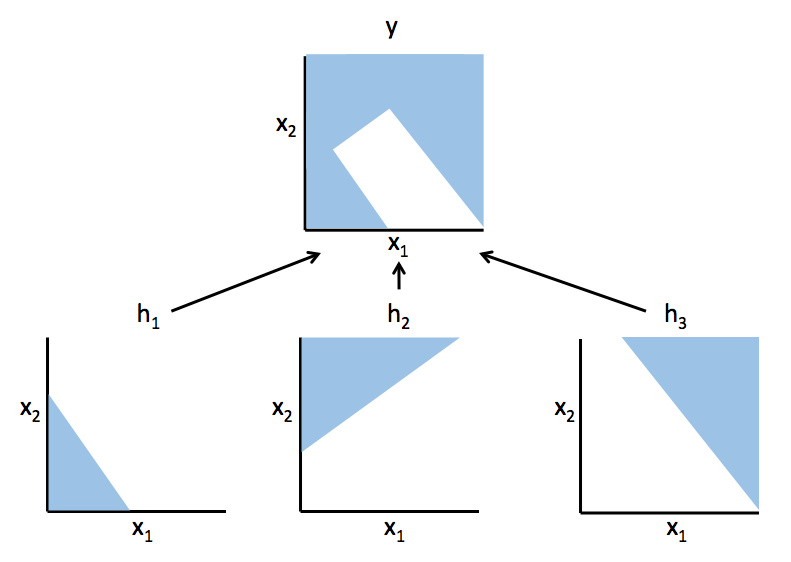
\includegraphics[scale=0.2]{figs/twolayer_nonlinearity}}
\pause
\item Backpropagation is an efficient way to train 2-layer nets:
\bi
	\item Similar to SGD for 1-layer net, just more chaining in gradient
	\pause
	\item General form: update $w_{ij}$ by ${\color{red} \delta_j} {\color{blue} x_i}$, and ${\color{red} \delta_j}$ is scaled/weighted sum of errors from outgoing layers
\ei
\pause
\item Ideally, we want even deeper architectures
\bi
	\pause
	\item But Backpropagation becomes ineffective due to vanishing gradients 
	\item Deep Learning comes to the rescue! (next lecture)
\ei
\ee
\end{frame}










%%%%%%%%%%%%%%%%%%%%
\begin{frame}[allowframebreaks]
\frametitle{References}
\bibliographystyle{apalike}
\bibliography{mybib}
\end{frame}

\end{document}
